\head{Декабрь}{Переводная самостоятельная работа. Уровень 1 $\Rightarrow$ уровень 2.}

\section{Подсчёт рёбер, двудольные графы. Обходы.}

\begin{figure}[H]
\begin{minipage}{0.19\linewidth}
    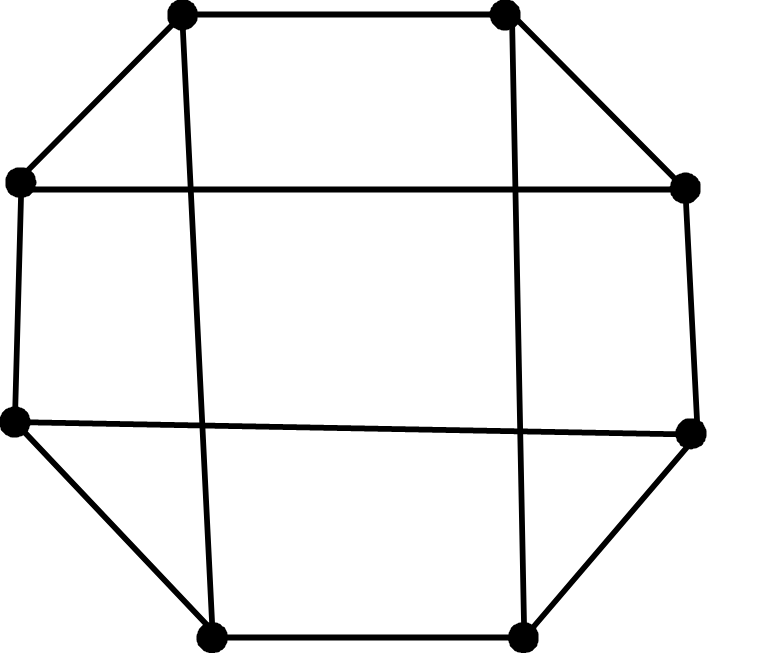
\includegraphics[width=0.95\columnwidth]{img/10.4.0 img1.png}
\end{minipage}
    \hfill
\begin{minipage}{0.8\linewidth}
    \begin{thm}
        Является ли граф, приведённый на рисунке, двудольным?
    \end{thm}
    \begin{thm}
        На конкурсе по математике было 20 задач. На разбор пришло 20 школьников. Известно, что каждый школьник решил ровно две задачи и каждую задачу решило ровно два школьника. Докажите, что можно так организовать разбор задач, что каждую задачу расскажет решивший её школьник.
    \end{thm}
\end{minipage}
\end{figure}

\begin{figure}[H]
\begin{minipage}{0.6\linewidth}
    \begin{thm}
        На рисунке изображён план дома. Линиями отмечены стены. (см. рис.) Можно ли провести по дому освещение (протянуть один провод) так, чтобы при этом просверлить каждую стену ровно один раз?
    \end{thm}
    \begin{thm}
        В одном учреждении каждый сотрудник выписывает две газеты, каждую газету выписывают пять человек, каждую пару газет выписывает только один человек. Сколько человек в учреждении и сколько они выписывают газет?
    \end{thm}
\end{minipage}
    \hfill
\begin{minipage}{0.39\linewidth}
    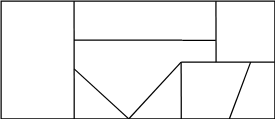
\includegraphics[width=0.95\columnwidth]{img/10.4.0 img2.png}
\end{minipage}
\end{figure}

\begin{thm}
    Докажите, что если граф двудольный, то все его циклы состоят из чётного числа рёбер.
\end{thm}

\begin{thm}
    Докажите, что если в графе все циклы чётной длины, то этот граф -- двудольный.
\end{thm}

\begin{thm}
    В стране Карликании 11 городов. Известно, что среди любых трёх из них хотя бы двое ещё не соединены авиалинией. Докажите, что в стране не более 30 авиалиний.
\end{thm}

\begin{thm}
    Докажите, что независимое множество максимально тогда и только тогда, когда оно доминирующее.
\end{thm}

\begin{thm} $^*$
    Докажите теорему из листка с теорией, воспользовавшись подсказкой.
\end{thm}

\begin{thm}
    В шахматном турнире в один круг участвуют 11 шахматистов. В настоящее время среди любых трёх из них хотя бы двое еще не сыграли. Доказать, что сыграно не более 30 партий.
\end{thm}

\begin{thm}
В классе каждый мальчик дружит ровно с двумя девочками, а девочка -- ровно с тремя мальчиками. Ещё известно, что в классе 31 пионер и 19 парт. Сколько человек в классе?
\end{thm}

\begin{thm}
    В народной дружине 100 человек. В каждый вечер на дежурство выходят трое. Докажите, что нельзя составить график дежурств таким образом, что любые два человека будут дежурить вместе ровно один раз.
\end{thm}

\begin{thm}
    Кружок по астрономии проводился в школе 20 раз. На каждое занятие приходило 6 человек. Известно, что никакие два школьника не встречались более чем на одном занятии. Доказать, что не менее 21 школьника посетили кружок.
\end{thm}

\begin{figure}[H]
    \begin{minipage}{0.89\linewidth}\setlength{\parindent}{1.5em}
        \begin{thm}
             В некоторые 16 клеток доски 8×8 поставили по ладье. Какое наименьшее количество пар бьющих друг друга ладей могло при этом оказаться?
        \end{thm}
        \begin{thm}
            На рисунке изображён план парка и его окрестностей, линиями отмечены заборы. (см. рис.) Можно ли прогуляться по парку так, чтобы при этом перелезть через каждый забор ровно один раз?
        \end{thm}
    \end{minipage}
\hfill
    \begin{minipage}{0.1\linewidth}
        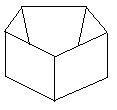
\includegraphics[width=0.95\columnwidth]{img/10.4 figure.png}
    \end{minipage}
\end{figure}

\begin{thm}
    В футбольном турнире участвует 20 команд. После того, как все команды провели по две игры, организаторы турнира решили разбить их на три дивизиона, но так, чтобы в одном дивизионе не было команд, уже игравших друг с другом. Всегда ли они смогут это сделать? (Подсказка. Вспомните теорему о циклических графах)
\end{thm}

\begin{thm}
    На $n$ карточках с двух сторон написаны числа от 1 до $n$ по два раза каждое. Докажите, что карточки можно положить на стол так, чтобы сверху каждое из чисел было написано ровно один раз.
\end{thm}

\begin{thm} $^*$
    В некоторой стране из каждого города выходит по три железные дороги. Две компании хотят их все приватизировать. Антимонопольный комитет требует, чтобы из каждого города выходили дороги обеих компаний. Докажите, что компании могут договориться так, чтобы требование антимонопольного комитета было выполнено.
\end{thm}

\begin{thm}
    Сварщик варит решетку размером 4×4 из кусков ломаных. Сможет ли он это сделать, если у него есть а) 5 ломаных длины 8; б) 8 ломаных длины 5? \textit{(Форма ломаных может быть различной)}
\end{thm}